\renewcommand{\thepage}{}
\chapter{Feasibility Analysis and Requirements Determination}
\thispagestyle{empty}
\pagestyle{fancy}
\lhead{\small \bf  Chapter 3: Feasibility Analysis and Requirements Determination}
\rhead{}
\chead{}
\renewcommand\thepage{\arabic{page}}
 \setcounter{minitocdepth}{1}
\minitoc
\clearpage
\section{Introduction}
\lettrine[lines=2,lhang=0.44,lraise=0,loversize=0.08,findent=-0.11em,slope=0.6em]%
{T}{} he $IG�$ application is intended to be used by various businesses, and especially pharmaceutical companies, private banks and medical offices. It has therefore been conceived to meet the needs of each business to which it is addressed. The majority of the needs are common to all kinds of usage, however specific ones depend on each business. Our application has been designed and developed to be open and configurable enough to adapt to the businesses for which it was tested as well as other.
\paragraph*{}
A specification is the definition of the project: a statement of the problem, not the solution. Normally, the specification contains errors, ambiguities, misunderstandings and enough rope to hang you and your entire team. Thus before embarking upon a long time of activity working on the wrong project, one must assume that a numbty\footnote{a numbty is a person whose brain is totally numb. In this context, numb means "deprived of feeling or the power of unassisted activity"; in general, a numbty needs the stimulation of an electric cattle prod to even get to the right office in the morning. Communication with numbties is severely hampered by the fact that although they think they know what they mean (which they do not), they seldom actually say it, and they never write it down. And the main employment of numbties world-wide is in creating project specifications. You must know this - and protect your team accordingly.} was the chief author of the received specification and one must read, worry, revise and ensure that everyone concerned with the project (from originator, through the workers, to the end-customer) is working with the same understanding. The outcome of this deliberation is a written definition of what is required, by when; and this must be agreed by all involved.
\paragraph*{}
The work on the specification can be seen as the first stage of Quality Assurance since one is looking for and countering problems in the very foundation of the project - from this perspective the creation of the specification clearly merits a large investment of time. From a purely defensive point of view, the agreed specification also affords a protection against the numbties who have second thoughts, or new ideas, half way through the project.
\section{Identification of the business requierements}
\paragraph*{}
The specifications have been provided by The Stradefi-SA team and discussed with the appropriate persons. After analyzing the specifications, we identified the following business requirements:
\begin{itemize}[font=\color{black}, label=\ding{98}]
\item The nodes can be individuals, objects or any abstract entity.
\item The edges represent relationships between the nodes. These relationships can be unilateral, bilateral or double.
\item Nodes as well as relations have properties and attributes. The application populates the necessary properties attached to the nodes and edges for the radial representation of the information received from the JSON files.
\item Nodes and relations are specified in JSON file. The use of XML is possible in order to make the $IG�$ Application open to other usages and other businesses.
\item The application explores the JSON files, identifies the nodes and relationships and builds a radial graph.
\item The nature of the relationship (unilateral, bilateral or multiple) is a characteristic that the application is able to analyze and represent.
\item Documents may  be associated to nodes (underlying document). They are stored in a document management system. The document path or ID is a property of the node.
\item When a node is selected it becomes the node of interest. It is automatically centered (becomes the center of the radial graph).
\item Some (significant) properties related to a given node, can be shown in a Panel, when the node is clicked.
\item A relation might be described in a document (underlying document). The document is therefore associated to the relation and stored in a document  management system. The document path or ID is a property of the relation.
\item The application calculates the distance between nodes. Distance defines, for instance, the degree of relation between two persons. The distance is defined with a level (it is anticipated that five levels are sufficient):
\begin{itemize}[font=\color{black}, label=\ding{227}]
\item Level 1 means that the two nodes are directly connected.
\item Level 2 means that the two nodes are connected via and 3rd node.
\item Etc.
\end{itemize}
\item The application is able to organize and arrange the nodes on the appropriate orbits.
\item The $IG�$ application allowing navigating through the radial graph:
\begin{itemize}[font=\color{black}, label=\ding{227}]
\item By double clicking on a node, an extra menu appears with extra feature:
 \begin{itemize}
  \item Display property in an extra pane
  \item Make this node as "selected", this action redraws the graph.
  \end{itemize}
\end{itemize}
\item Showing Mouse over (mouse only) the node or over the relation displays the property of the object (either in pop up or in another window)
\item A "mouse click" (touch also) makes the display permanent until a close on the top right cross.
\item A "double click" (touch again) opens the underlying document (click on the node, click on the relation).
\item The document opens in a separate Web onglet.
\item The user can create a graph in two ways:
	\begin{itemize}[font=\color{black}, label=\ding{227}]
	\item Scriptural: he fills a form with fields, drop down list...
	\item Graphical: capability to draw a line on a graph to create a relation, key in the properties and attaching documents
	\end{itemize}
\item The document is attached to the relation. If the document is uploaded from the PC, the document is loaded to the content management implying metadata to be filled manually or automatically
\item The user is able to change the display of nodes and edges upon their own properties.
\item The user can save a graph and its setting. 
\end{itemize}
\section{Analysis of business requirements}
\paragraph*{}
The business requirements presented in the last paragraph are the result of several discussions that we had inside the team. The specifications of the $IG�$ application expressed lots of requirements however we considered only some of them that seemed to us the most significant ones. For the detailed list of selected requirements, please refer to the table IV.1. These final requirements was considered as the product backlog and we started the design and the implementation if the $IG�$ application on the basis of this backlog. In this chapter we present the different use cases and activity diagrams corresponding to the items that have been developed in the current version of $IG�$.
\subsection{The general Use Case}
\paragraph*{}
The following diagram represents the overall view of $IG�$ application. The user can create a new graph or act on an existing one. He can select a node in order to move it, to access to its properties and attributes and  to update them. The user can select a relation, to see its properties and to modify them. 
\newpage
\begin{figure}[h]
\centering
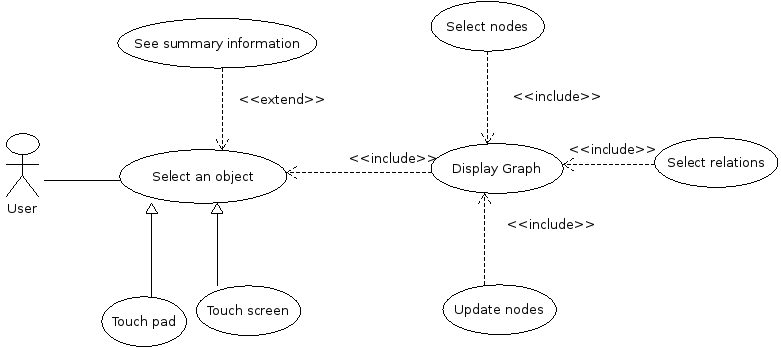
\includegraphics[scale=0.75, frame]{GeneralUseCase.png}
\caption{General use case diagram}
\end{figure}
\subsection{Use Case: Display a Graph}
\paragraph*{}
This functionality allows the end user to visualize his object and their relationships by rendering a radial graph.
\begin{itemize}[font=\color{black}, label=\maltese]
\item A user interface dialogue allows to select an object, in order to display the corresponding Radial Graph;
\item When the mouse cursor goes over an object, a summary of its information is shown in a tooltip;
\item By selecting an object, the corresponding Radial Graph is displayed.
\end{itemize}
\newpage
\subsubsection{Use Case description}
\begin{table}[h]
\begin{tabular}{|p{5cm}|p{10cm}|}
\hline
\textbf{Title} & Display Graph\\
\hline
\textbf{Actor} & User\\
\hline
\textbf{Pre condition} & The user must be logged in and the list of the objects he can access to, is not empty.\\
\hline
\textbf{Post Condition} & This step ends when the Graph is displayed\\
\hline
\textbf{Description} & \begin{itemize}
\item The list of the available objects, that the user can access to, is shown in a dialog.
\item By passing the mouse cursor over an object a summary of its properties is shown.
\item the user selects an object by clicking on it and the corresponding radial graph is displayed
\item the user can access, either  to the summary of the properties of any node or the detailed attributes of the node of interest
\end{itemize} \\
\hline
\end{tabular}
\caption{textual description }
\label{Textual description}
\end{table}
\subsubsection{Use Case diagram}
\paragraph*{}
The figure III.2 presents the detailed use case diagram of the document visualization module.
\begin{figure}[h]
\begin{center}
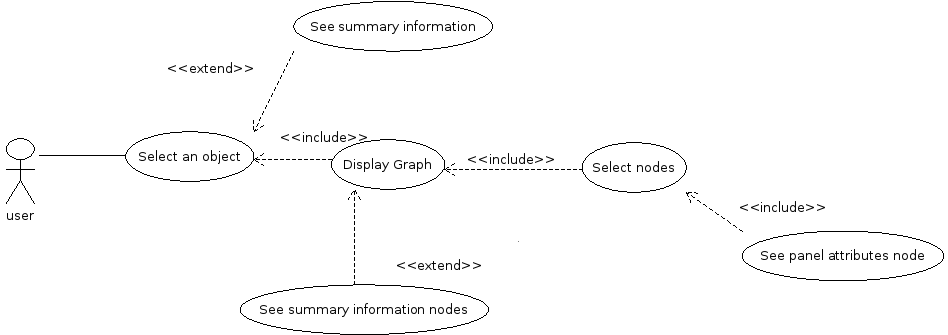
\includegraphics[scale=0.6, frame]{DisplayGraphUC.png}
\end{center}
\caption{Display Graph Use Case}
\end{figure}
\subsubsection{The "Display Graph" activity diagram}
\paragraph*{}
The user connects to $IG�$ application, the different objects  he can access to are listed in the screen.
The list may be empty if the user has no access rights to any object. If the list is not empty, he can select an object and visualize the corresponding radial graph. The default node of interest is centered. The user may select a different node that becomes the new node of interest and therefore centered. He can access, either  to the summary of the properties of any node or the detailed attributes of the node of interest.
\begin{figure}[h]
\begin{center}
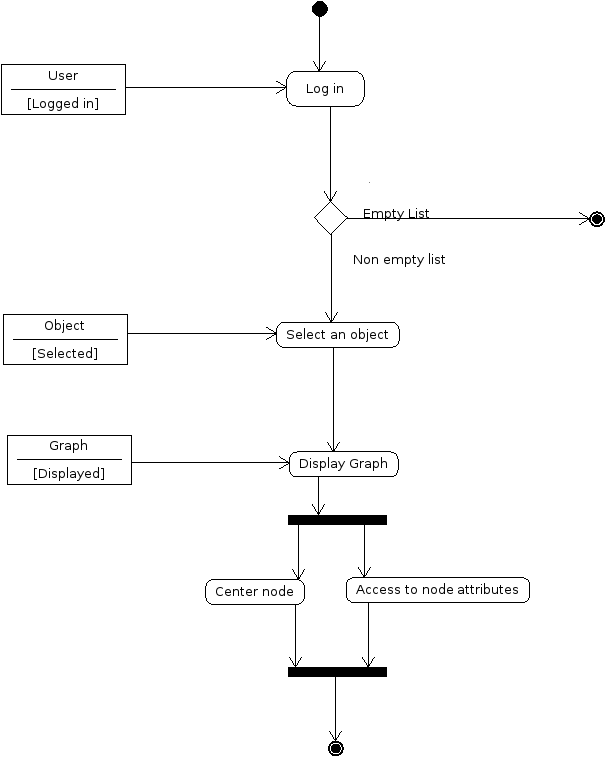
\includegraphics[scale=0.8, frame]{DisplayGraphAD.png}
\end{center}
\caption{Display Graph Activity Diagram}
\end{figure}
\newpage
\subsubsection{Use Case: Update Node}
\paragraph*{}
This use case allows users to change or update a given node proprieties\\
\begin{table}[h]
\begin{tabular}{|p{5cm}|p{10cm}|}
\hline
\textbf{Title} & Update nodes \\
\hline
\textbf{Actor} & User \\
\hline
\textbf{Pre Condition}& Only the node the interest may be updated. The user must be logged in \\
\hline
\textbf{Post Condition} & This step ends when the user comfirms or cancels the modification\\
\hline
\textbf{Description}& The user selects "modify node" menu item. The detailed attributes of the node of interest are shown in a popup window. He, then can modify one or more attributes. The updating of attributes may be confirmed or canceled.\\
\hline
\end{tabular}
\caption{textual description "Update Nodes"}
\label{Textual description of update nodes}
\end{table}
\subsubsection{Use Case diagram }
\begin{figure}[h]
\begin{center}
\includegraphics[scale=0.8, frame]{UpdateNodesUC.png}
\end{center}
\caption{Use case Update node}
\end{figure}
\subsubsection{The "Update Nodes" Activity Diagram}
\paragraph*{}
The activity diagram (fig. 3.8) details the "node update use case". The user must be connected, then he selects the "update node" item in the general menu. This item applies only on the node of interest and displays its attributes. Each attributes is put in an input text that the user may modify. After updating the appropriate attributes the user can save his modifications or cancel the operation. The confirmation of the actions results in the updating of the JSON file.
\newpage
\begin{figure}[h]
\begin{center}
\includegraphics[scale=0.8, frame]{UpdateNodesDA.png}
\end{center}
\caption{Node Update Activity Diagram}
\end{figure}
\section{Conclusion}
\paragraph*{}
This chapter results from the detailed analysis of the specifications given by Stradefi SA. The business requirements have been clearly identified and validated. Each requirements has been specified and designed. We therefore presented a use case and an activity diagram for the most important requirements. Each of them has also been validated with Stradefi SA. Some of the requirements were not completely expressed and one decided to delay their analysis and design; this will be detailed in the next chapter that discusses the methodology and the project plan.

